% This is based on the LLNCS.DEM the demonstration file of
% the LaTeX macro package from Springer-Verlag
% for Lecture Notes in Computer Science,
% version 2.4 for LaTeX2e as of 16. April 2010
%
% See http://www.springer.com/computer/lncs/lncs+authors?SGWID=0-40209-0-0-0
% for the full guidelines.
%
\documentclass{llncs}
\usepackage{geometry}
\usepackage{indentfirst}
\usepackage{float}
\usepackage{graphicx}
\usepackage{multicol}
\usepackage{amssymb, amsmath}
\usepackage{booktabs, array, multirow}
\usepackage{color}
\newcommand{\todo}[1]{\textcolor{red}{@TODO: #1}}


\begin{document}
\pagestyle{plain}
\title{Understand Amazon Wish List -- User Shopping Preference and Privacy Exposer}
%
\titlerunning{Amazon}  % abbreviated title (for running head)
%                                     also used for the TOC unless
%                                     \toctitle is used
%
\author{Yue Li\inst{1} \and Nan Zheng\inst{1}
Haining Wang\inst{2} \and Kun Sun\inst{1}\and Zhaoliang Duan\inst{1} \and Cheng Li\inst{1}}
%
\authorrunning{Yue Li et al.} % abbreviated author list (for running head)
%
%%%% list of authors for the TOC (use if author list has to be modified)
\tocauthor{Yue Li, Nan Zheng, Haining Wang, Kun Sun, Zhaoliang Duan, and Cheng Li}
%
\institute{College of William and Mary\\
\email{yli@cs.wm.edu}
\and University of Delaware}
\maketitle              % typeset the title of the contribution

\begin{abstract}
The malware used for IV\&V was based on actual malware source code that
performs a variety of functions (e.g., key logging, clip board stealing, etc). The
source code was acquired by DARPA, combined into different executables, and
compiled using various flags into Windows 32-bit binaries. There are three data
sets associated with this data, TC1, TC2 and TC3. TC1 contains 50 samples
of malware and eight components. TC2 contains same eight components, but
added compiler variations (e.g., optimizations on or off) to produce a data set
of 250 malware samples. Finally, TC3 contained 27 total components over 500
malware samples, where 250 of the malware samples are the same ones from
TC2.
\end{abstract}


\section{Introduction}
Entering the era of big-data, Internet has been largely extended to be data-rich. Network users are prone to expose their private information in public websites inadvertently \cite{frankowski2006you}, making themselves face the threat of information leakage. To study how the information bundle can be used to threat user privacy, we investigate user profile and their Wish Lists in Amazon, unveiling its user behaviour exposure threat and potential privacy leakage. 

We collected complete profile and wish lists information of over 20,000 users in Amazon. Based on the data, we conduct measurement study on user behaviour. Our measurement study concentrates on user shopping preference, which are organized in 3 dimensions — 1)What to buy 2)When to buy 3)Product prices users are willing to pay. 

In summary, we have the following contribution:
\begin{enumerate}
\item  We collected a large number of user profile (over 20,000)and their Wish Lists by web scraping. We analyzed Wish Lists of each of the users we collected and present interesting observations. Specifically we compare the user preference in different regions and gender. In addition, shopping peaks and pits through a year are also investigated. Surprisingly we found that people do not always like to shop in holidays.
\item We conduct a preliminary study on user privacy information identification using Wish Lists. We used Support vector machine (SVM) to train and test data. The ground truth is retrieved from user list-description in their Amazon profiles. We assert that Wish Lists are sufficient to sell user privacy information out.
\end{enumerate}

\section{Data Collection}
\subsection{Data Structure and Methodology}
Amazon Wish Lists reside in it's user profiles. One can view a user's Wish List in his/her profile. There are also other objects in user profiles, such as Reviews, Activities, and Tagged items. However, these objects are beyond the scope of this paper. We omit the discussion of these objects. 

Figure~\ref{data_struct} shows the data hierarchy in our study. As seen from Figure~\ref{data_struct}, user profiles provide basic information of the users —- name or nickname, birthday, location, and list-description. list-description is plain text keyed in by the users, which is usually used to briefly introduce the Wish Lists and the users. An example is "I LOVE music! Buy me a CD!" or "Son of Sue and Kevin, brother of Roger, husband of Kathy. I moved from Milton Keynes, England to Smithfield, North Carolina, USA on 8/8/2000 and recently moved from there to the Raleigh/Garner border in the same state". Note that the birthday information does not include the year, and the location includes solely state and city, which makes the data less privacy sensitive. However, we can still sense some information leakage through the list-description. Our first example above shows the hobby of a user -- Music. Our second example exposes much more personal information -- Parents' names, brother's name, marriage status, wife name, moving history, etc. Note that birthday, location, and list-description are optional therefore a profile may not always has these privacy information available. Amazon profiles are always public accessible and wish lists are public accessible by default. 
\begin{figure}[H].
\centering
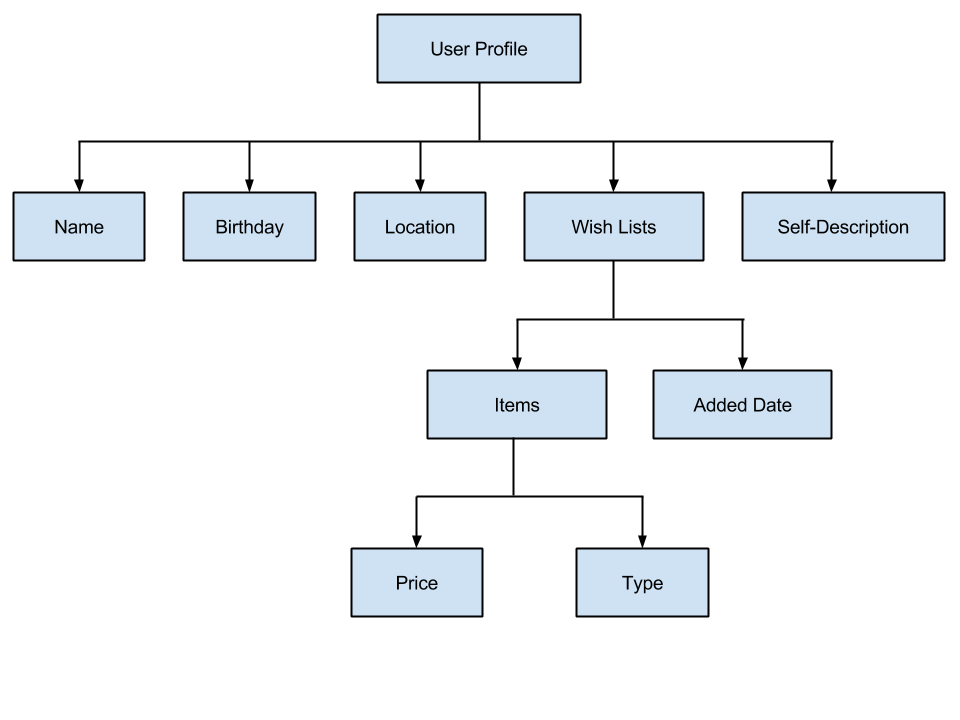
\includegraphics[width=.75\textwidth]{data_struct.png}
\caption{data hierarchy}.
\label{data_struct}
\end{figure}
To conduct sound measurement, large number of data are desired. A natural way is to crawl Amazon by web scraping. Therefore we used a crawler to download Amazon web pages and retrieve useful information in these pages. Note that Amazon did provide API named Product Advertising API to owners of other websites to help embedding Amazon service in their websites. However, we insist on using web scraping over Product Advertising API for 2 major reasons -- 1) Product Advertising API does not provide "type" information of items, which is essential in our analysis. 2) There is a 2,500 requests/hour limit on an initial API account. Using few API accounts do not boost the speed while signing up for more accounts require much more effort.

The data collection process consists of 3 steps.
First we search a common name in the search engine provided by Amazon \cite{searcheng}, which is shown in Figure~\ref{searcheng}. Amazon will return at most 2016 (24 per page for 84 pages) users that are associated with a name. Note that the search engine usually gives notice that hundreds of thousand users are found, but only the first 2016 users are viewable. The results returned include user profile link, user Wish List names, links to the lists, and list-descriptions.

\begin{figure}[H].
\centering
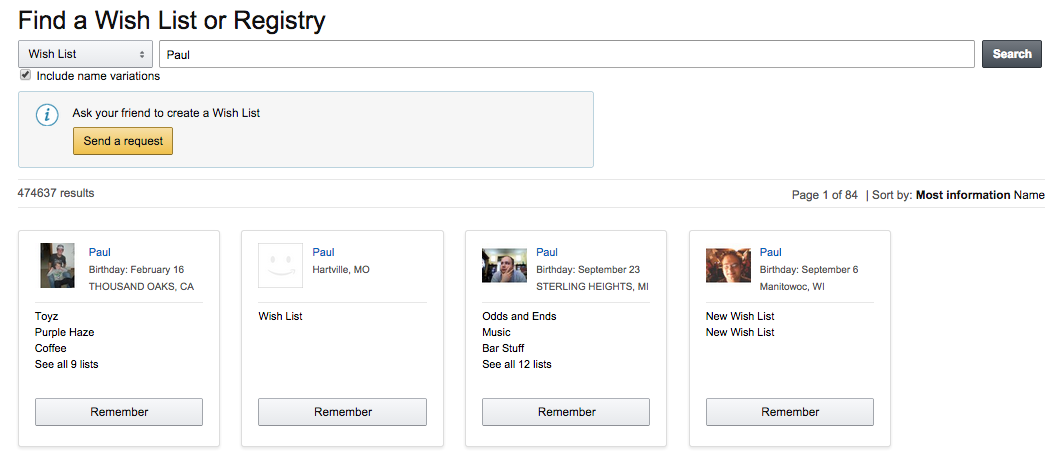
\includegraphics[width=.85\textwidth]{searcheng.png}
\caption{Amazon Search Engine}.
\label{searcheng}
\end{figure}

Afterwards, we find the items inside each of the wish list in a target user. Given that the Wish List URLs and IDs have been recorded, we downloaded pages of the user's Wish Lists. We then record each item in each of the Wish List. However, in this step we have little information about the item (Only the name, and the date the item is added). We obtain the URLs to the item page and visit them to retrieve more information in the next step. Note that currently we do not find a upper limit on the number of items inside a wish list and some items may no longer exist in Amazon so the link may fail or be greyed out. 

\begin{figure}[H].
\centering
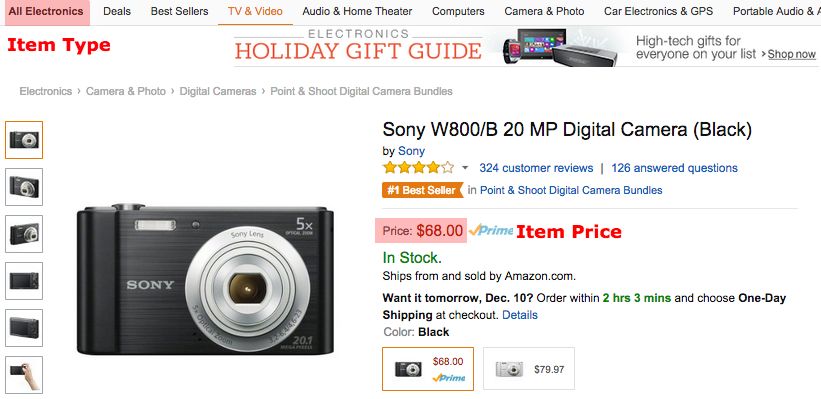
\includegraphics[width=.85\textwidth]{item.png}
\caption{A web page of Amazon product}.
\label{itempage}
\end{figure}

Finally We retrieve detailed information for each item. We visit all the item URLs and download the product pages, hopefully (but not with 100\% success rate) we can find the price and categories of the items. One example of the product web pages is shown in Figure~\ref{itempage}. In Figure~\ref{itempage}, we can easily find the item type and the item price (In red box). The information is retrieved from the source code of the page by finding the content in certain HTML tags. Note that there may not always be only one price for an item. For example, for the same item, there can be prices from different retailers. There are also differences between new ones and used ones. We record only the most obvious price -- the price the first retailer and in this case, the amazon prime price, and we only record prices of new items. Not always we can find the price of an item. There are multiple reasons -- 1)There is no price on the page 2)The price is rendered using client-side javascript, which will not be run when crawling the web pages 3)Network failures. However, having few items without prices has little impact on our analysis.



\subsection{Data Overview}
In the first step of the data collection process. We searched the top 600 common names (300 males \cite{mnames} and 300 females \cite{fnames} in Amazon, which theoretically returns over 1,200,000 users. However, different searchings may return the same user. For example, if a man names "James Paul", he will be returned when searching either "James" or "Paul". Therefore the returned names have some repetition. As a result, we actually collected 967,603 unique users.Their profile information and wish list links are stored in our database. However, we do not collect the wish lists and items of all the users returned. As we are also interested in personal information of a user, we only collect the wish lists and items of users who potentially have information leakage -- users with list-description. As collecting all users with list-description are very time-consuming, we only collect data that can sufficiently derive solid results in the second and third steps. To this end, we collected 20099 users with list-descriptions, together with all the items and wish lists. Besides the users, we collected 48,848 wish lists and 3,320,211 items, among which 1448806 are unique. The size of the data is approximately 1GB. 

\section{Data Analysis}
\subsection{Statistics}
We use our data in different ways. The very first step is to conduct fundamental measurements on the dataset. We wish to help people have a basic understanding about the usage of wish lists and to what extent do the users expose their personal information in Amazon. 

For all 967,603 users, there are totally 2,121,173 wish lists recorded, which means each user has 2.2 wish lists in their Amazon profile. Among the 967,603 users, 104846 (10.8\%) of them have input their list-descriptions. In addition, there are 280,328 (29.0\%) users who have filled their birthday information, 221,298 (22.9\%) users who have filled their location information, and 150,004 (15.5\%) users who have filled both the birthday and address information. In addition, among the 104,846 users who have self descriptions, 94,284 (89.9\%) of them have birthday information and 59,731 (57\%) of them have address information. Although the birthday and address information is not particular (birthday only shows month and day and address only shows the city and state), we can still see that a non-trivial portion of users put their personal information on their amazon profiles. What is more, most of the people who have filled out a list-description have exposed their birthday and address information. One can argue that the open birthday information may be of some use (so others can prepare birthday presents). However, the address information is meaningless for a user to expose to the public. Even for gift givers, Amazon will not show the address of the receiver. In this case, users are giving out their personal information meaninglessly. Our findings agree with \cite{frankowski2006you}, which states that users tend to expose their personal information in open websites. 

As we did not collect a complete dataset for all the users, we then analyze only the users we have collected so far. In the completed user dataset, we have 20,099 users and 48,848 wish lists. We can see that the average number of wish lists a user have is 2.43 in the completed dataset, which is a little higher than that of the whole dataset. We believe the little gap is reasonable because the users who have filled the list-descriptions seems using Amazon more so they are more prone to input birthday information, address information, and products in their profiles. 

The maximum number of wish list in a user profile in our data set is 184. We further analyze the distribution of the number of wish list a user has, which is shown in Figure~\ref{avglist}

\begin{figure}[H]
\minipage{0.3\textwidth}
  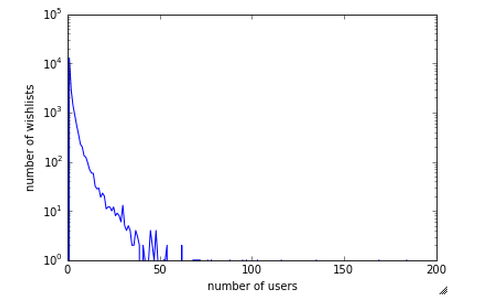
\includegraphics[width=\linewidth]{avglist.png}
  \caption{Number of lists the users have}
  \label{avglist}
\endminipage\hfill
\minipage{0.3\textwidth}%
  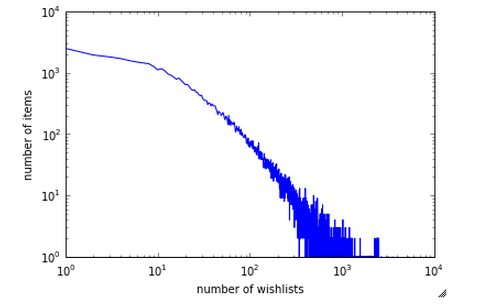
\includegraphics[width=\linewidth]{avgitem.png}
  \caption{Number of items the lists have}
  \label{avgitem}
\endminipage\hfill
\minipage{0.3\textwidth}%
  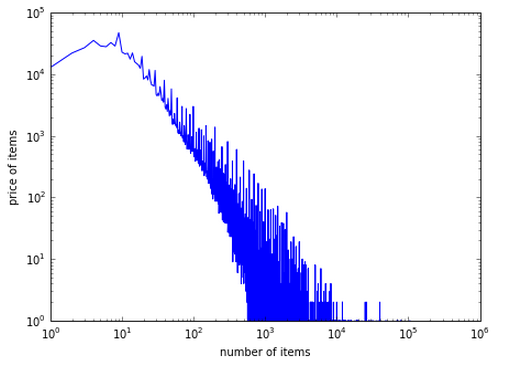
\includegraphics[width=\linewidth]{avgprice.png}
  \caption{Item Price}
  \label{avgprice}
\endminipage
\end{figure}

Similarly, we analyze the distribution of the number of wish list a user has, which is shown in Figure~\ref{avgitem}. The maximum number of items in a wish list in our dataset is 5,238 and the average number of items in a wish list is 68. 

As we can see from the two figures, both the distributions of wish lists and items follow a similar trend -- most of the users have around average number of wish lists and most wish lists have average number of items. However, there are a few of the data points are far from the average. 

Another thing we are interested in is the price of the items. The average price of all the items 47.16 US dollars. The distribution of the prices are shown in Figure~\ref{avgprice}. The price figure is more irregular than the Figure~\ref{avglist} and Figure~\ref{avgitem} because the data points in Figure~\ref{avgprice} is much more than the other 2 figures.


So far we have learned the basic usage of Wish Lists, there is still some distance from understanding user shopping preference and pattern. We will learn the difference between different regions in the US. These information are valuable to advertisers and commercial companies. 

\todo{ADD NATION-WIDE PREFERENCE}
\subsection{User preference in different regions}
We analyze the user preference in different regions, which are -- east coast, west coast, and middle of the US according to Wikipedia \cite{east}\cite{west}. It is natural to consider that people may have different shopping preference in different regions. We quantitatively show the differences in this section as well as presenting interesting observations. The average price of east coast, west coast, and middle of US is \$25.69, \$27.33 and \$24.87 accordingly. As the price in Amazon will not be different for users from different regions, our result indicates that the price sensitivity is highest in middle area of the US, and is lowest in the west coast area. It agrees with the common knowledge -- the average income in coastal area is higher than the middle area, and the west coast is higher than the east coast. 

We further look into the detailed The top 20 preferences for people from east coast is shown in Table~\ref{tb:east}. The top 20 preferences for people from west coast is shown in Table~\ref{tb:west} and the top 20 preferences for people from middle of the US is shown in Table~\ref{tb:mid}

\begin{table}[!htbp]
\caption{EAST COAST USER PREFERENCE}
\label{tb:east}
\begin{tabular}{lllll}
Rank & Item Type          & Number of Items & Percentage of Items & Average Price(\$) \\
1 & Books & 210205 & 41.44\% & \$6.19 \\
2 & Movies \& TV & 63648 & 12.55\% & \$17.11 \\
3 & CDs \& Vinyl & 46726 & 9.21\% & \$9.75 \\
4 & Buy a Kindle & 25859 & 5.10\% & \$9.77 \\
5 & Toys \& Games & 25542 & 5.04\% & \$41.73 \\
6 & Sports \& Outdoors & 15619 & 3.08\% & \$48.73 \\
7 & Video Games & 14819 & 2.92\% & \$31.01 \\
8 & Amazon Fashion & 11379 & 2.24\% & \$45.26 \\
9 & All Electronics & 9054 & 1.79\% & \$123.91 \\
10 & Home Improvement & 8929 & 1.76\% & \$60.18 \\
11 & Kitchen \& Dining & 8209 & 1.62\% & \$53.59 \\
12 & Home \& Kitchen & 6702 & 1.32\% & \$58.87 \\
13 & Camera \& Photo & 5647 & 1.11\% & \$314.25 \\
14 & Computers & 5516 & 1.09\% & \$119.79 \\
15 & Health \& Personal Care & 4302 & 0.85\% & \$48.56 \\
16 & Digital Music & 3776 & 0.74\% & \$0.00 \\
17 & Patio, Lawn \& Garden & 3642 & 0.72\% & \$88.11 \\
18 & Automotive & 3478 & 0.69\% & \$62.53 \\
19 & Musical Instruments & 3157 & 0.62\% & \$154.15 \\
20 & Cell Phones \& Accessories & 2867 & 0.57\% & \$37.65 \\
\end{tabular}
\end{table}

\begin{table}[!htbp]
\caption{WEST COAST USER PREFERENCE}
\label{tb:west}
\begin{tabular}{lllll}
Rank & Item Type          & Number of Items & Percentage of Items & Average Price(\$) \\
1 & Books & 145939 & 41.99\% & \$6.10 \\
2 & Movies \& TV & 46266 & 13.31\% & \$16.52 \\
3 & CDs \& Vinyl & 33981 & 9.78\% & \$8.85 \\
4 & Buy a Kindle & 18072 & 5.20\% & \$9.98 \\
5 & Toys \& Games & 16351 & 4.70\% & \$40.03 \\
6 & Sports \& Outdoors & 9191 & 2.64\% & \$57.02 \\
7 & Video Games & 8708 & 2.51\% & \$30.75 \\
8 & Amazon Fashion & 7223 & 2.08\% & \$85.60 \\
9 & Home Improvement & 7002 & 2.01\% & \$66.70 \\
10 & All Electronics & 6756 & 1.94\% & \$147.81 \\
11 & Kitchen \& Dining & 4905 & 1.41\% & \$51.04 \\
12 & Home \& Kitchen & 4448 & 1.28\% & \$71.36 \\
13 & Camera \& Photo & 4267 & 1.23\% & \$322.14 \\
14 & Computers & 3908 & 1.12\% & \$117.42 \\
15 & Digital Music & 2921 & 0.84\% & \$0.00 \\
16 & Health \& Personal Care & 2801 & 0.81\% & \$40.73 \\
17 & Automotive & 2383 & 0.69\% & \$63.70 \\
18 & Musical Instruments & 2022 & 0.58\% & \$128.10 \\
19 & Cell Phones \& Accessories & 1878 & 0.54\% & \$36.98 \\
20 & Patio, Lawn \& Garden & 1808 & 0.52\% & \$108.02 \\
\end{tabular}
\end{table}

\begin{table}[!htbp]
\caption{MIDDLE OF US USER PREFERENCE}
\label{tb:mid}
\begin{tabular}{lllll}
Rank & Item Type          & Number of Items & Percentage of Items & Average Price(\$) \\
1 & Books & 362966 & 43.96\% & \$8.27 \\
2 & Movies \& TV & 112737 & 13.65\% & \$16.11 \\
3 & CDs \& Vinyl & 75685 & 9.17\% & \$9.19 \\
4 & Buy a Kindle & 43510 & 5.27\% & \$9.37 \\
5 & Toys \& Games & 42419 & 5.14\% & \$37.36 \\
6 & Video Games & 24587 & 2.98\% & \$29.93 \\
7 & Sports \& Outdoors & 20101 & 2.43\% & \$50.90 \\
8 & Amazon Fashion & 16635 & 2.01\% & \$76.39 \\
9 & Home Improvement & 12977 & 1.57\% & \$69.84 \\
10 & All Electronics & 12009 & 1.45\% & \$124.05 \\
11 & Kitchen \& Dining & 11292 & 1.37\% & \$45.95 \\
12 & Home \& Kitchen & 10321 & 1.25\% & \$59.15 \\
13 & Camera \& Photo & 7488 & 0.91\% & \$338.27 \\
14 & Computers & 6993 & 0.85\% & \$125.67 \\
15 & Digital Music & 6965 & 0.84\% & \$0.00 \\
16 & Health \& Personal Care & 5458 & 0.66\% & \$37.70 \\
17 & Automotive & 5021 & 0.61\% & \$66.18 \\
18 & Patio, Lawn \& Garden & 4666 & 0.57\% & \$101.79 \\
19 & Musical Instruments & 4245 & 0.51\% & \$151.28 \\
20 & Grocery \& Gourmet Food & 3915 & 0.47\% & \$18.99 \\
\end{tabular}
\end{table}

From the tables we have the following observations.

\begin{enumerate}
\item Books are dominating the wish lists in these areas with all over 40\% of the items being books.

\item There are more reading lovers in the middle area of the US. Although the price sensitivity is highest in the middle area, people there are more likely to accept higher price on books, given that the average price of books in the middle area is 33.6\% and 35.6\% higher than east and west coast correspondingly. 

\item Besides books, entertainment also plays an important roles. Movies\& TV and CDs \& Vinyl rank second and third in the wish lists. In fact, in all the 3 areas, the top categories are basically the same, which means that people from different regions are likely to buy similar types of products. 

\item There are still differences in user shopping preference. For example, people from west and middle are willing to pay much more in fashion (clothing, shoes, etc) than people from east (west -- \$85.6, middle -- \$76.4, east -- \$45.3). On the other hand, people from east are willing to pay more in Health \& Personal care (around 20\% higher in average price). Besides, people from coastal areas seem purchasing more electronics and computers than the middle area. Besides, People from west are more tolerable to high prices in Sports \& Outdoors products. 

\end{enumerate}
In conclusion, these information is valuable to companies to promote their products and advertisers to find the price preferences for different users. 

\subsection{Holidays}
In this section we measure how the items are added in the wish lists during holidays and normal days. As there are many unofficial or regional holidays, in our study only nation-wide federal holidays are considered. There are totally 10 qualified holidays. These holidays (http://www.usa.gov/citizens/holidays.shtml) and the date of the holidays are listed in Table~\ref{tb:holiday}



\begin{table}[!ht]
\centering
\caption{U.S Federal Holidays}
\label{tb:holiday}
\begin{tabular}{p{2cm}p{6cm}p{6cm}p{2cm}}
& New Year's Day & January 1 & \\
& Birthday of Martin Luther King, Jr. & third Monday in January & \\
& Washington's Birthday & third Monday of February & \\
& Memorial Day & last Monday of May & \\
& Independence Day & July 4 & \\
& Labor Day & first Monday of September & \\
& Columbus Day & second Monday in October & \\
& Veterans Day & November 11 & \\
& Thanksgiving Day & fourth Thursday in November & \\
& Christmas Day & December 25 & \\
\end{tabular}
\end{table}

Next we analyze the data in 2 dimensions. First, We measure the items added in these holidays and compare the average items added in holidays and average items added in normal days. Then we compare the added items among different holidays. When calculating items added in a certain holiday, we consider the nearest consecutive 5 days. That is to say, we include the previous 2 days and the next 2 days in our holiday shopping session. For example, the Christmas day is December 25. We will include December 23, December 24, December 25, December 26, December 27 in Christmas day calculation. As a result, calculate items added during a year in a little different manner -- we include the last 2 days in previous year because the 2 days are considered New Year's day. We do not include the first 2 days in the next year because there is no holidays in the end of Decembers.


\subsubsection{Holidays and Normal Days}
According to our data, people start to add items in their wish lists since 1999. We analyze the items added in normal days and holidays in each year by calculating the average items added in the 2 groups. Table~\ref{tb:year} shows the detailed statistics.

\begin{table}[!htbp]
\centering
\caption{Items Added in Normal Days and Holidays}
\label{tb:year}
\begin{tabular}{lllll}
Year & Avg in Normal days & Avg in Holidays & Increase & Percentage \\
1999 & 3.60 & 5.74 & 2.14 & 59.4\% \\
2000 & 32.88 & 36.34 & 3.46 & 10.5\% \\
2001 & 77.42 & 76.60 & -0.82 & -1.1\% \\
2002 & 122.00 & 136.52 & 14.52 & 11.9\% \\
2003 & 156.00 & 166.32 & 10.32 & 6.6\% \\
2004 & 176.41 & 184.84 & 8.43 & 4.8\% \\
2005 & 297.15 & 315.36 & 18.21 & 6.1\% \\
2006 & 375.32 & 395.36 & 20.04 & 5.3\% \\
2007 & 417.15 & 455.06 & 37.91 & 9.1\% \\
2008 & 452.08 & 472.12 & 20.04 & 4.4\% \\
2009 & 511.98 & 540.14 & 28.16 & 5.5\% \\
2010 & 658.89 & 725.60 & 66.71 & 10.1\% \\
2011 & 921.30 & 1016.34 & 95.04 & 10.3\% \\
2012 & 1254.19 & 1402.52 & 148.33 & 11.8\% \\
2013 & 1773.25 & 1918.34 & 145.09 & 8.2\% \\
\end{tabular}
\end{table}

From Table~\ref{tb:year} we make the following observations:
\begin{enumerate}
\item The items added in wish lists increase year by year, no matter in normal days or holidays. We believe that the reason behind is that electric commercial gains its popularity.
\item There is increase in number of items added during holidays. The average increase rate is 10.89\%. However, as the data for year 1999 is not sufficient to be representative, we exclude year 1999 in our calculation and eventually we conclude that there is around 5.9\% increase in holidays. 
\item Generally people do buy more stuff during holidays. However, the increase is very limited. In 2001, the items added during holidays are even less than normal days. 
\end{enumerate}

To better illustrate the result, Figure~\ref{year} shows the items added in normal days and holidays (red line represents normal days and blue lines represent holidays). 

\begin{figure}[H]
\minipage{0.5\textwidth}
  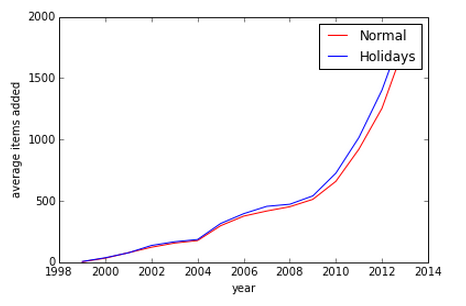
\includegraphics[width=\linewidth]{year.png}
  \caption{Number of items added in normal days and holidays}.
  \label{year}
\endminipage\hfill
\minipage{0.5\textwidth}%
  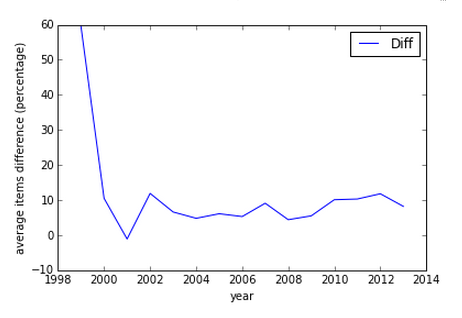
\includegraphics[width=\linewidth]{holiday.png}
  \caption{Increase from normal items }.
  \label{holiday}
\endminipage
\end{figure}

\subsubsection{Different Holidays}
Previously we compared the shopping difference between holidays and normal days. We found that although people shop more in holidays, the increase is not that much. Our findings are against common impression that people do shop a lot in holidays, especially Thanksgiving and Christmas. We realized that it is rough to group all national holidays together to compare to normal days. We believe that holidays are also different from each other. For example people tend to shop more in Thanksgiving and Christmas. Therefore we compare different holidays in our study. Similarly, we include the last 2 days in the previous year in our analysis. There are 10 national holidays as introduced before. We again calculate the average number of items added in the nearest consecutive 5 days and compare to the average number of normal days. 

We use the data from year 1999 - 2013 and the year 2013 solely. We wish to show both the average case(from 1999-2013) and the current trend (only year 2013). We do not use data from Year 2014 because during the time of the study, the years 2014 has not been finished. Note that when computing the average item number added in normal days, we leave out all the holidays instead of simply leaving out the one that is being analyzed. The result is shown in Figure~\ref{alldiffholiday} for 1999-2013 and Figure~\ref{diffholiday} for the year 2013. In Figure~\ref{diffholiday}, The x-axis indicate the holidays accordingly (0-New Year's day, 1-Birthday of Martin Luther King, Jr, 2-Washington's Birthday, 3-Memorial Day, 4-Independence Day, 5-Labor Day, 6-Columbus day, 7-Veterans Day, 8-Thanksgiving day, 9-Christmas day).


\todo{A better graph with self-explanatory x axis}
\begin{figure}[H]
\minipage{0.5\textwidth}
  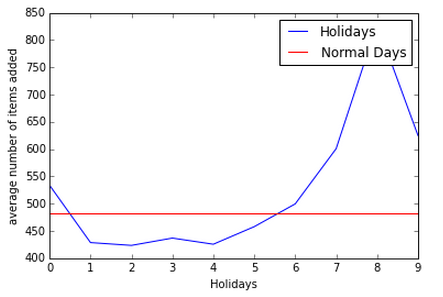
\includegraphics[width=\linewidth]{alldif.png}
\caption{Different Holidays through 15 years}.
\label{alldiffholiday}
\endminipage\hfill
\minipage{0.5\textwidth}%
  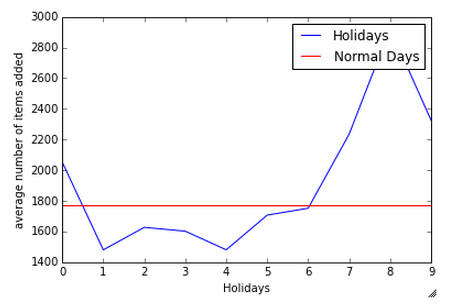
\includegraphics[width=\linewidth]{diff.png}
\caption{Different Holidays in 2013}.
\label{diffholiday}
\endminipage
\end{figure}


According to Figure~\ref{alldiffholiday} and Figure~\ref{diffholiday}, we find that holidays have huge difference between each other. In addition, we make the following observations:
\begin{enumerate}
\item The 2 figures match very well, which means that people do not tend to change their shopping behaviors at least during a short period of time. 
\item Some of the holidays are not much different from normal days (For example, Columbus Day). What is more, some of the holidays make the people less willing to add items in their wish lists. 
\item New Year's day, Veterans day, Thanksgiving, and Christmas day are 4 holidays that have quite obvious shopping increase. The result indicates that people tend to buy more stuff during the 4 holidays. The increase rate is 4.1\%, 25.2\%,72.8\%, and 30.2\% accordingly for all 15 years we analyzed. 
\item Among the 4 holidays, Thanksgiving day is the most shopping appealing holiday, which is 72.8\% higher than normal days. It is reasonable because people always get considerable discount during thanksgiving days. Christmas is the second most shopping appealing holiday because people always need to buy presents during Christmas.
\item At the first glance it is surprising that 4 holidays -- Birthday of Martin Luther King. Jr, Washington's Birthday, Memorial Day, Independence Day, and Labor day -- clearly have even less items added to user Wish Lists. The drop percentage is 10.7\%, 11.8\%, 9.0\%, 11.3\%, and 4.6\%. One possible reason is that People are more likely to be involved in other activities other than shopping during these holidays. 3 out of the 4 holidays are memorial days. Certainly these days are considered not good for shopping. 
\end{enumerate}

\section{Privacy Information Identification}

From our measurement study, we have studies 3 dimensions of user shopping preference -- 1)What to buy 2)When to buy 3)Price.

From our study of shopping preference difference, it has been clear that different people have different shopping preference. One question is: Can we identify user personal information from the their Wish Lists. That is to say, Items added in Wish Lists have potential to leak personal information. We explore the possibility using machine learning to help identify user personal information from their Wish Lists.
\subsection{Information in list-description}
To successfully identify the user personal information. One challenge we face is how to obtain the ground truth of the user. There are several possible ways to find out the result. First, Services such as yahoo people search can be used as ground truth at a reasonable monetary cost. We can input the name and location information in the search engine to identify a user. Second, similar to the first approach, we can search people in online social networks such as Facebook or Twitter. Third, we can use the user list-description as the ground truth. Users sometimes expose personal information in their list-description and we can take advantage of it.

The first approach does not really provide an accurate result since the information given is not rigorous enough to identify the exact person. If wrongly identified, it has much negative impact on the identification process, which is by itself not very accurate already. The second approach is similar to the first one. It is even more inaccurate. Due to the unreliable nature of the first 2 approaches, we took the third approach. Besides the accuracy, collecting ground truth from list-descriptions have the benefit of not depending on external data source. Recall that we collect items for only users with list-descriptions. All our 20,099 users collected have list-descriptions. Note that there are also limitations for the third approach. For example, the list-description is plain-text, making it hard to process and analyze. Secondly, there may not always be useful information in list-descriptions.

We assume that everybody is telling the truth in the list-descriptions. If somebody is lying, we do not have a way to identify it. However, it is meaningless for a user to lie in list-descriptions since lying there will not bring them any benefit. If a user concerns his/her privacy, he/she can simply leave the list-description blank instead of lying.

Among the users who have list-descriptions, 233,595 words are found (44,387 punctuations are excluded). The average number of words in list-descriptions is 11.6. We can see that the list-descriptions are not long -- basically the length of a normal sentence. While there are scattered long list-description (the longest list-description has 682 words), more than half of the list-descriptions have length less than or equal to 6 (10,592 out of 20,099). And only 29.9\% of the list-descriptions have over 10 words. Considering that there are even less words that carry information, One possible consequence is that there might not be enough information in one list-description to identify personal information.

Next we retrieve information from list-descriptions. 

One way to retrieve information is to search the keyword. If a keyword appears in one user's self-description, there is high probability that the user is related to the keyword. For example, if a keyword "college" appears in the self-description, the user is likely to have a college degree. 

We used Stanford Part-of-Speech (POS) tagger \cite{toutanova2003feature} to tag the user list-descriptions to retrieve useful information. There are a number of tags a word can belong to. However, we only focus on noun-family words (with tag NN, NNS, NNP, and NNPS in Stanford POS tagger). The reason behind is that most of the nouns carry certain amount of information while most of other words do not carry useful information. 

There are totally 95,359 out of all 233,595 words (around 40.8\%) belonging to the noun family. The ratio of nouns is quite large. The most frequent ones are listed in Table~\ref{tb:freq}

\begin{table}[!ht]
\centering
\caption{FREQUENT NOUNS IN list-descriptionS}
\label{tb:freq}
\begin{tabular}{p{3cm}p{3cm}p{3cm}p{3cm}p{3cm}}
 & Rank & Item Type & frequency & \\
 & 1 & s & 1498 &  \\
 & 2 & love & 1327 &  \\
 & 3 & m & 1314 &  \\
 & 4 & university & 1098 &  \\
 & 5 & music & 1095 &  \\
 & 6 & list & 1064 &  \\
 & 7 & books & 1001 &  \\
 & 8 & school & 659 &  \\
 & 9 & movies & 652 &  \\
 & 10 & t & 628 &  \\
 & 11 & games & 593 &  \\
 & 12 & things & 553 &  \\
 & 13 & college & 495 &  \\
 & 14 & stuff & 443 &  \\
 & 15 & work & 419 &  \\
 & 16 & fan & 411 &  \\
 & 17 & wish & 389 &  \\
 & 18 & video & 380 &  \\
 & 19 & history & 371 &  \\
 & 20 & photography & 353 &  \\
\end{tabular}
\end{table}

From Table~\ref{tb:freq} We can see that except for meaningless single characters ("s" and "m" in this case), the noun family words carry some information of a user. The information involves hobbies (such as music, books, movies, etc) and education level (such as university, college). These words can be used as keywords in the information retrieval step. On the other hand, if we look into the verbs, we will find the most popular 20 verbs are "is",  "am",  "have",  "are",  "live",  "be",  "love",  "buy",  "want",  "enjoy",  "know",  "used",  "do",  "don",  "get",  "married",  "go",  "went",  "read",  "loves",  and "was". Except "married", the other words can not assist us to find any useful information about a user.
\subsection{Information Identification}
We do personal information identification on a subset of users who have more than 30 items in their wish lists in our dataset. We filter part of the users out because they do not have sufficient information in their Wish Lists. After the filtering, we have 13,464 users as our target users. We choose users with certain keywords in their list-descriptions in the user pool. We use the portion of different types of products,  in user wish lists as input to the classifier. Therefore we have an input vector of length of 50. We use SVM classifier to train and test the data. 80\% of our data is used as training data and the rest of 20\% of the data as testing data. The personal information identification process is binary, which means that we use only 2 classes in each identification cycle. The reasons for having only 2 classes. It is reasonable to have 2 classes in a classifier. We intend to answer questions like "Is he a professor?", "Does he have a university diploma" or "Does he like hiking?". A prediction of the answer is very helpful in identifying a user. We try 2 different types of personal information -- 1) gender 2)hobbies

\subsection{gender}
There are only 2 genders in general, it is natural to have only 2 classes. To save the training resource while maintaining high representation, we chose 389 males and 168 females as our dataset. We used the first 80\% person as the training set and the rest as the test set. The ground truth comes from the name of the users. We identify a user "male" if this user is using a male name in the profile. females are identified using a similar approach. As a result, the success rate to classify whether a given user is a male or female is around 84\%.
We can see that the classifier works pretty well in the case of gender, which means that given only the Wish List information of a user, we can identify whether this user is male or female with pretty high certainty.

\subsection{Hobbies}
Afterwards, We use hobbies as examples, we choose all pairs of hobbies in the top 20 nouns. 7 keywords are selected. They are -"music", "books", "movies", "games", "video", "history", and "photography" and try to differentiate users between any pair of them. The success rate between any pair of them is shown in Table~\ref{tb:hobby}

\begin{table}[!ht]
\centering
\caption{Success Rate of Hobbies}
\label{tb:hobby}
\begin{tabular}{llllllll}
            & music & books & movies & games & video & history & photography \\
music       & NA    & 0.506 & 0.653  & 0.713 & 0.691 & 0.772   & 0.743       \\
books       & 0.506 & NA    & 0.631  & 0.667 & 0.647 & 0.526   & 0.807       \\
movies      & 0.653 & 0.631 & NA     & 0.617 & 0.617 & 0.762   & 0.662       \\
games       & 0.713 & 0.667 & 0.617  & NA    & 0.521 & 0.776   & 0.703       \\
video       & 0.691 & 0.647 & 0.617  & 0.521 & NA    & 0.777   & 0.700       \\
history     & 0.772 & 0.526 & 0.762  & 0.776 & 0.777 & NA      & 0.680       \\
photography & 0.743 & 0.807 & 0.662  & 0.703 & 0.700 & 0.680   & NA         
\end{tabular}
\end{table}

We can see that the success rate can be high (80.7\%) or even no better than guessing (50.6\%). Such big variance may be due to the relativity of different hobbies. When 2 hobbies are not much related, we can find the success rate be usually higher than 70\%. For example, "history" has very limited relativity to other hobbies except for "books". We can see from the table that history has higher success rate except for the "books" entry because history relates to books pretty much. It is difficult to have further increase in success rate because people often have more than 1 hobbies. Therefore one person may belong to both group, which will have quite negative impact on the result.

We conclude that wish lists are helpful to identify a user's hobby. However, depending solely on wish lists are not a very reliable option to identify user hobbies. 

\section{Limitation and Future Work}
\subsection{Limitation}
There are limitations in our work. We discuss the limitations and possible consequences from these limitations. 
\begin{enumerate}
\item The data may be biased. The user wish lists are not always public -- users have the ability to change the accessibility of their wish lists (although the default is public). Therefore privacy-aware users may choose to publicize some of their wish lists while keep other wish lists from strangers. Besides, users may choose not to share certain items in their wish lists. For example, privacy-sensitive items such as pregnancy test, firearm-related products, and medicine \& drugs. In our work we can only retrieve the product in public wish lists. The data may not be accurately representative of one users' shopping behavior.

\item When data of price is involved, some products are ignored. We have mentioned that the price cannot always be retrieved. There are multiple reasons and some of them cannot be easily solved such as price not being displayed or javascript being used for displaying the price. Besides, some prices do not accurately reflect the user's preference because there might be multiple prices (from various retailers, used ones or new ones), and we do not know which one does the user prefer. We take only the new one and the first retailer's price. 

\item When doing personal information identification. We actually do not have complete ground truth. Using the keyword approach will give us a group of people with certain features. However, we cannot identify a large enough group without the features. For example, searching "engineer" gives us a group of engineers, however, we do not know whether the users not mentioning "enginner" in their list-descriptions are engineers or not. This lack of complete ground truth may have big negative impact on the success rate of our information identification step.

\end{enumerate}
\subsection{Future Work}
We discuss future work that can be done.
\begin{enumerate}
\item Use possibly better information retrieval method. In our project, the information retrieval step is straight-forward -- we search the keywords in users' list-descriptions to label the users. It works with relatively high accuracy. However, this method is a little too strict so that not many users are selected for a certain class. One way to improve our result is to use a better information retrieval method. We can possibly obtain more users for a specific group while maintaining relatively high accuracy. It will provide more stable data and probably more well-trained SVM.
\item There are 2 ways to improve the user personal information identification process. The first way is to improve the accuracy of the classification step. The second way is to use our method as a filter to filter out irrelevant users and use some other strategies to do further identification.
\end{enumerate}
\todo{MORE RELATED WORK, CONCLUSION, AND REFERENCES}
\section{Related Work}


There are a large amount of works that have been done to learn plain text. \cite{de2001mining} mines e-mail content for author identification. They study an extended set of email document features, which include structure, linguistic patterns, etc. They use SVM learning algorithm to differentiate the authors of emails. \cite{pang2002thumbs}presented algorithm for mining users' opinions of an item from their reviews of the items, classifying documents in overall sentiment. They use keywords appearing in the user comments of an item to infer whether the user like this item or not and to what extend do they like/dislike the item.

\cite{Lee:2010:USS:1835449.1835522} does statistical analysis of the properties of spam profiles collected from social network communities for creating spam classifiers to actively filter out existing and new spammers. \cite{dave2003mining} describes the system infrastructure, identify the unique properties of list of product attributes and develops a method for automatically distinguishing between positive and negative reviews in Movie Lens to link forum posts to mentioned items. \cite{kraft2007mashing}attempts to do on a set of Amazon wish lists spiders from web. They started by doing a wish lists search of people names(first names and nicknames from the baby names databases) and then retrieve the results linking to the wish lists of the first 25 matches. 

\section{Conclusion}
In this project, we investigate Amazon public wish lists, where users store their desired products. We collect over 20,000 users' complete profile and wish list items and take a 2-step approach to analyze our data. The first step is that we try to measure the user behavior from their wish lists. We answer the following questions: 1) Are users from different regions follow the same shopping patter? Is there any difference among people in different regions? 2) Is the common belief that people shop more during special date, especially holidays reflected in Amazon wish list? Our result shows that although people from different regions are following a general shopping behavior, they still have differences. Interesting observations such as east coast people are less willing to pay high price on clothing are presented in our measurement result. Furthermore, we investigate user shopping preference in holidays and normal days. We found that people do shop more in holidays, but the increase is not significant. We then explore different holidays through a year, we found that although there are holidays that people shop much more than normal days, there are over half of the holidays that have no increase or even lower shopping records.  The second step we take is trying to identify personal information from the items in a user's wish list. We retrieve our ground truth information from the data using a keyword approach -- searching a keyword in users' list-descriptions to divide users into different classes. This approach works well because it is accurate while it labels sufficient people for machine learning purpose. We use SVM to train and classify the data obtained from the information retrieval step. We examined 2 types of personal information -- gender and hobbies. We use the first 80\% data for training and the rest 20\% of data for testing. The gender classification gives a good success rate of over 80\%. However, identifying hobbies does not always achieve a satisfying success rate. This accuracy is not good enough to identify users' personal information. However, it can provide help when accuracy requirement is not high. It is also able to serve as a filter for a more complex identification tool.


%
% ---- Bibliography ----
%
\bibliographystyle{plain}

\bibliography{ref}

\end{document}
